%%%%%%%%%%%%%%%%%%%%%%%%%%%%%%%%%%%%%%%%%
% Programming/Coding Assignment
% LaTeX Template
%
% This template has been downloaded from:
% http://www.latextemplates.com
%
% Original author:
% Ted Pavlic (http://www.tedpavlic.com)
%
% Note:
% The \lipsum[#] commands throughout this template generate dummy text
% to fill the template out. These commands should all be removed when 
% writing assignment content.
%
% This template uses a Perl script as an example snippet of code, most other
% languages are also usable. Configure them in the "CODE INCLUSION 
% CONFIGURATION" section.
%
%%%%%%%%%%%%%%%%%%%%%%%%%%%%%%%%%%%%%%%%%

%----------------------------------------------------------------------------------------
%	PACKAGES AND OTHER DOCUMENT CONFIGURATIONS
%----------------------------------------------------------------------------------------

%\documentclass{article}
\documentclass[12pt]{article}
\usepackage{fancyhdr} % Required for custom headers
\usepackage{lastpage} % Required to determine the last page for the footer
\usepackage{extramarks} % Required for headers and footers
\usepackage[usenames,dvipsnames]{color} % Required for custom colors
\usepackage{graphicx} % Required to insert images
\usepackage{subcaption}
\usepackage{listings} % Required for insertion of code
\usepackage{courier} % Required for the courier font
\usepackage{amsmath}
\usepackage{framed}

% Margins
\topmargin=-0.45in
\evensidemargin=0in
\oddsidemargin=0in
\textwidth=6.5in
\textheight=9.0in
\headsep=0.25in

\linespread{1.1} % Line spacing

% Set up the header and footer
\pagestyle{fancy}
\lhead{\hmwkAuthorName} % Top left header
\chead{\hmwkClass\ (\hmwkClassTime): \hmwkTitle} % Top center head
%\rhead{\firstxmark} % Top right header
\lfoot{\lastxmark} % Bottom left footer
\cfoot{} % Bottom center footer
\rfoot{Page\ \thepage\ of\ \protect\pageref{LastPage}} % Bottom right footer
\renewcommand\headrulewidth{0.4pt} % Size of the header rule
\renewcommand\footrulewidth{0.4pt} % Size of the footer rule

\setlength\parindent{0pt} % Removes all indentation from paragraphs

%----------------------------------------------------------------------------------------
%	CODE INCLUSION CONFIGURATION
%----------------------------------------------------------------------------------------

\definecolor{mygreen}{rgb}{0,0.6,0}
\definecolor{mygray}{rgb}{0.5,0.5,0.5}
\definecolor{mymauve}{rgb}{0.58,0,0.82}

\lstset{ %
  backgroundcolor=\color{white},   % choose the background color
  basicstyle=\footnotesize,        % size of fonts used for the code
  breaklines=true,                 % automatic line breaking only at whitespace
  captionpos=b,                    % sets the caption-position to bottom
  commentstyle=\color{mygreen},    % comment style
  escapeinside={\%*}{*)},          % if you want to add LaTeX within your code
  keywordstyle=\color{blue},       % keyword style
  stringstyle=\color{mymauve},     % string literal style
}

%----------------------------------------------------------------------------------------
%	DOCUMENT STRUCTURE COMMANDS
%	Skip this unless you know what you're doing
%----------------------------------------------------------------------------------------

% Header and footer for when a page split occurs within a problem environment
\newcommand{\enterProblemHeader}[1]{
%\nobreak\extramarks{#1}{#1 continued on next page\ldots}\nobreak
%\nobreak\extramarks{#1 (continued)}{#1 continued on next page\ldots}\nobreak
}

% Header and footer for when a page split occurs between problem environments
\newcommand{\exitProblemHeader}[1]{
%\nobreak\extramarks{#1 (continued)}{#1 continued on next page\ldots}\nobreak
%\nobreak\extramarks{#1}{}\nobreak
}

\setcounter{secnumdepth}{0} % Removes default section numbers
\newcounter{homeworkProblemCounter} % Creates a counter to keep track of the number of problems
\setcounter{homeworkProblemCounter}{0}

\newcommand{\homeworkProblemName}{}
\newenvironment{homeworkProblem}[1][Problem \arabic{homeworkProblemCounter}]{ % Makes a new environment called homeworkProblem which takes 1 argument (custom name) but the default is "Problem #"
\stepcounter{homeworkProblemCounter} % Increase counter for number of problems
\renewcommand{\homeworkProblemName}{#1} % Assign \homeworkProblemName the name of the problem
\section{\homeworkProblemName} % Make a section in the document with the custom problem count
\enterProblemHeader{\homeworkProblemName} % Header and footer within the environment
}{
\exitProblemHeader{\homeworkProblemName} % Header and footer after the environment
}

\newcommand{\problemAnswer}[1]{ % Defines the problem answer command with the content as the only argument
\noindent\framebox[\columnwidth][c]{\begin{minipage}{0.98\columnwidth}#1\end{minipage}} % Makes the box around the problem answer and puts the content inside
}

\newcommand{\homeworkSectionName}{}
\newenvironment{homeworkSection}[1]{ % New environment for sections within homework problems, takes 1 argument - the name of the section
\renewcommand{\homeworkSectionName}{#1} % Assign \homeworkSectionName to the name of the section from the environment argument
\subsection{\homeworkSectionName} % Make a subsection with the custom name of the subsection
\enterProblemHeader{\homeworkProblemName\ [\homeworkSectionName]} % Header and footer within the environment
}{
\enterProblemHeader{\homeworkProblemName} % Header and footer after the environment
}

%----------------------------------------------------------------------------------------
%	NAME AND CLASS SECTION
%----------------------------------------------------------------------------------------

\newcommand{\hmwkTitle}{Assignment 2} % Assignment title
\newcommand{\hmwkDueDate}{Friday, Mar 15, 2019} % Due date
\newcommand{\hmwkClass}{CSC412} % Course/class
\newcommand{\hmwkClassTime}{LEC 0101} % Class/lecture time
\newcommand{\hmwkAuthorName}{Zhongtian Ouyang} % Your name
\newcommand{\hmwkAuthorID}{1002341012} % Your name

%----------------------------------------------------------------------------------------
%	TITLE PAGE
%----------------------------------------------------------------------------------------

\title{
\vspace{2in}
\textmd{\textbf{\hmwkClass:\ \hmwkTitle}}\\
\normalsize\vspace{0.1in}\small{Due\ on\ \hmwkDueDate}\\
\vspace{0.1in}
\vspace{3in}
}

\author{\textbf{\hmwkAuthorName}\\ \textbf{\hmwkAuthorID}}

\date{(collaborate with Yihao Ni)} % Insert date here if you want it to appear below your name

%----------------------------------------------------------------------------------------\
\begin{document}

\maketitle
\clearpage

%----------------------------------------------------------------------------------------
%	Common Tools
%----------------------------------------------------------------------------------------
%\begin{framed}
%\begin{lstlisting}[language=matlab]
%\end{lstlisting}
%\end{framed}

% \begin{bmatrix}
%0.5 & 0.6 \\ 
%0.7 & 0.8
%\end{bmatrix}

%\begin{figure}[h!]
%\centering
%\includegraphics[width=0.6\linewidth]{q10a.png}
%\label{fig:q10a}
%\end{figure}\\

%\begin{figure*}[!ht]
%\begin{subfigure}{.5\textwidth}
% \centering
%  \includegraphics[width=.5\linewidth]{p4_1.JPG}
%  \caption{Full set}
%  \label{fig:sfig1}
%\end{subfigure}
%\begin{subfigure}{.5\textwidth}
% \centering
%  \includegraphics[width=.5\linewidth]{P4_2.JPG}
%  \caption{Two each}
%  \label{fig:sfig2}
%\end{subfigure}%
%\caption{Part4 (a)}
%\label{fig:p4a}
%\end{figure*}

%\sum_{n=1}^{\infty} 2^{-n} = 1
%\prod_{i=a}^{b} f(i)

%\begin{equation}
%\begin{split}
%1+2+3+4+8x+7 & =1+2+3+4+4x+35 \\
%& \Rightarrow x=7
%\end{split}
%\end{equation}

%----------------------------------------------------------------------------------------
The code for this assignment is written in Python 3
\clearpage
%----------------------------------------------------------------------------------------
%	PROBLEM 1
%----------------------------------------------------------------------------------------

% To have just one problem per page, simply put a \clearpage after each problem
\begin{homeworkProblem}
(a)
$$L(\theta) = \prod_{i=1}^{10000} P(\mathbf{x}^{(i)}|c, \theta_c) = \prod_{i=1}^{10000} \prod_{d=1}^{784}\theta_{cd}^{x^{(i)}_d}(1-\theta_{cd})^{(1-x^{(i)}_d)}$$
\begin{equation}
\begin{split}
\hat\theta_{cd} &= \frac{num\ of\ data\ that\ are\ digit\ c\ and\ d^{th}\ pixel\ is\ present}{num\ of\ data\ that\ are\ digit\ c}\\
&=\frac{\sum_{i=1}^{10000} x_d^{(i)} \land (label^{(i)} == c)}{\sum_{i=1}^{10000}(label^{(i)} == c)} 
\end{split}
\end{equation}

(b)\\
$$
argmax_{\hat\theta}\frac{P(data|c, \theta_c = \hat\theta_c) P(\theta_c = \hat\theta_c)}{P(data|c)} = argmax_{\hat\theta_c}P(data|c, \theta_c = \hat\theta_c) P(\theta_c = \hat\theta_c)
$$
Since the prior for each $\theta$ is Beta(2,2),
$$
f(\theta; 2, 2) = \frac{\theta^{2-1}(1-\theta)^{2-1}}{B(2,2)} = \frac{\theta(1-\theta)}{B(2,2)} \propto \theta(1-\theta)
$$
$$
P(data|c, \theta_c = \hat\theta_c) = \prod_{i=1}^{10000}P(\mathbf{x}^{(i)}|c, \theta_c = \hat\theta_c) = \prod_{i=1}^{10000}\prod_{d=1}^{784}\hat\theta_{c^{(i)}d}^{x^{(i)}_d}(1-\hat\theta_{c^{(i)}d})^{(1-x^{(i)}_d)}
$$
We can find seperately the $\theta_{cd}$ value for each c, d that would maxmize the terms including that $\theta_{cd}$.\\
For an arbitray c,d value, let $N_c$ be the number of samples that are digit c. Let $N_{cd}$ be the number of samples that are digit c and the dth pixel is white.\\ Collecting the terms from $P(data|c, \theta_c = \hat\theta_c)$, we get:
$$\theta_{cd}^{N_{cd}}(1-\theta_{cd})^{N_c-N_{cd}}$$
Collecting the terms from $P(\theta_c = \hat\theta_c)$, we get:
$$\theta_{cd}(1-\theta_{cd})$$
Let:
$$F = \theta_{cd}^{N_{cd}}(1-\theta_{cd})^{N_c-N_{cd}}\theta_{cd}(1-\theta_{cd}) = \theta_{cd}^{N_{cd}+1}(1-\theta_{cd})^{N_c-N_{cd} + 1}$$
$$log(F) = (N_{cd}+1)log(\theta_{cd}) + (N_c-N_{cd} + 1)log(1-\theta_{cd})$$
$$\frac{d}{d\theta_{cd}}log(F)  = \frac{N_{cd}+1}{\theta_{cd}} - \frac{N_c-N_{cd} + 1}{1-\theta_{cd}}$$
Find $\hat\theta_{cd}$ by solving the following:
$$\frac{N_{cd}+1}{\hat\theta_{cd}} - \frac{N_c-N_{cd} + 1}{1-\hat\theta_{cd}} =0$$
$$\hat\theta_{cd} = \frac{N_{cd}+1}{N_c+2}$$
\clearpage

(c)
\begin{figure}[h!]
\centering
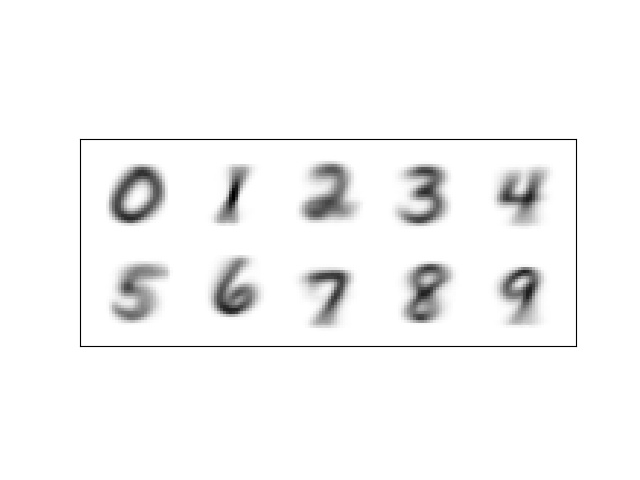
\includegraphics[width=0.6\linewidth]{q1c.jpg}
\label{fig:q1c}
\end{figure}

(d)\\
\begin{equation}
\begin{split}
&\ log(p(c|\mathbf{x},\boldsymbol{\theta}, \pi))\\
&=log(\frac{p(\mathbf{x}, c|\boldsymbol{\theta}, \pi)}{p(\mathbf{x}|\boldsymbol \theta)})\\
&=log (\frac{p(c|\pi)p(\mathbf{x}|c, \theta_c)}{\sum_{c1=0}^{9}p(\mathbf{x}|c1, \theta_{c1})})\\
&= log(p(c|\pi)) + log(p(\mathbf{x}|c, \theta_c)) - log(\sum_{c1=0}^{9}p(\mathbf{x}|c1, \theta_{c1}))\\
&= log(\pi_c) + log( \prod_{d=1}^{784}\theta_{cd}^{x_d}(1-\theta_{cd})^{(1-x_d)}) - log(\sum_{c1=0}^{9} \prod_{d=1}^{784}\theta_{(c1)d}^{x_d}(1-\theta_{(c1)d})^{(1-x_d)})\\
&= log(\pi_c) + \sum_{d=1}^{784}(x_dlog(\theta_{cd})+ (1-x_d)log(1-\theta_{cd})) - log(\sum_{c1=0}^{9} \prod_{d=1}^{784}\theta_{(c1)d}^{x_d}(1-\theta_{(c1)d})^{(1-x_d)})\\
& \propto log(\pi_c) + \sum_{d=1}^{784}(x_dlog(\theta_{cd})+ (1-x_d)log(1-\theta_{cd}))
\end{split}
\end{equation}
Notice that the last part  $log(\sum_{c1=0}^{9}p(\mathbf{x}|c1, \theta_{c1}))$ is the same for any input argument c to the $log(p(c|\mathbf{x},\boldsymbol{\theta}, \pi))$. We can therefore ignore this part when we making predictions to avoid the underflow problem.\\

(e)\\
Notice that the average of log likelihood here ignore the part mensioned above.\\
Training set Average log likelihood: -172.3538233466875\\
Test set Average log likelihood: -173.04360309120443\\
Training set accuracy: 0.8398\\
Test set accuracy: 0.8372\\
\end{homeworkProblem}
%----------------------------------------------------------------------------------------
%	PROBLEM 2
%----------------------------------------------------------------------------------------

\begin{homeworkProblem}
(a)\\
True\\

(b)\\
False\\

(c)\\
generated digits are:[5 8 5 0 0 1 7 6 2 4]. The digits are randomly generated with a fixed seed to make sure the result is reproducible.
\begin{figure}[h!]
\centering
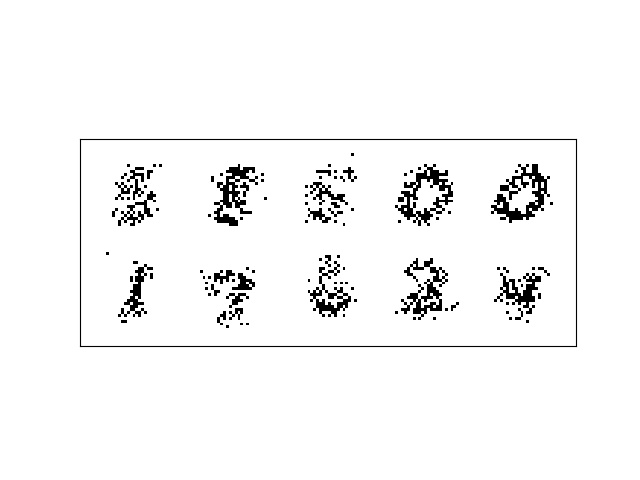
\includegraphics[width=\linewidth]{q2c.jpg}
\label{fig:q2c}
\end{figure}
\clearpage
(d)\\
\begin{equation}
\begin{split}
p(\mathbf{x}_{bottom}|\mathbf x_{top}, \boldsymbol \theta, \pi)
&= \frac{p(\mathbf{x}_{bottom}, \mathbf x_{top}|\boldsymbol \theta, \pi)}{p(\mathbf x_{top}|\boldsymbol \theta, \pi)}\\
&= \frac{p(\mathbf{x}|\boldsymbol \theta, \pi)}{p(\mathbf x_{top}|\boldsymbol \theta, \pi)}\\
&= \frac{\sum_{c=0}^{9} p(\mathbf{x}|c, \boldsymbol \theta, \pi)}{\sum_{c=0}^{9} p(\mathbf x_{top}|c, \boldsymbol \theta, \pi)}\\
&= \frac{\sum_{c=0}^{9} \prod_{d=1}^{784}\theta_{cd}^{x_d}(1-\theta_{cd})^{(1-x_d)}}{\sum_{c=0}^{9} \prod_{d=1}^{392}\theta_{cd}^{x_d}(1-\theta_{cd})^{(1-x_d)}}
\end{split}
\end{equation}

(e)\\
\begin{equation}
\begin{split}
p(\mathbf{x}_{i \in bottom}|\mathbf x_{top}, \boldsymbol \theta, \pi)
&= \frac{p(\mathbf{x}_{i \in bottom}, \mathbf x_{top}|\boldsymbol \theta, \pi)}{p(\mathbf x_{top}|\boldsymbol \theta, \pi)}\\
&= \frac{\sum_{c=0}^{9} p(\mathbf{x}_{i \in bottom}, \mathbf x_{top}|c, \boldsymbol \theta, \pi)}{\sum_{c=0}^{9} p(\mathbf x_{top}|c, \boldsymbol \theta, \pi)}\\
&= \frac{\sum_{c=0}^{9} p(\mathbf{x}_{i \in bottom}|c, \boldsymbol \theta, \pi)p(\mathbf x_{top}|c, \boldsymbol \theta, \pi)}{\sum_{c=0}^{9} p(\mathbf x_{top}|c, \boldsymbol \theta, \pi)},\ condionally\ independent\\
&= \frac{\sum_{c=0}^{9} \theta_{ci}^{x_i}(1-\theta_{ci})^{(1-x_i)} \prod_{d=1}^{392}\theta_{cd}^{x_d}(1-\theta_{cd})^{(1-x_d)}}{\sum_{c=0}^{9} \prod_{d=1}^{392}\theta_{cd}^{x_d}(1-\theta_{cd})^{(1-x_d)}}
\end{split}
\end{equation}

(f)
\begin{figure}[h!]
\centering
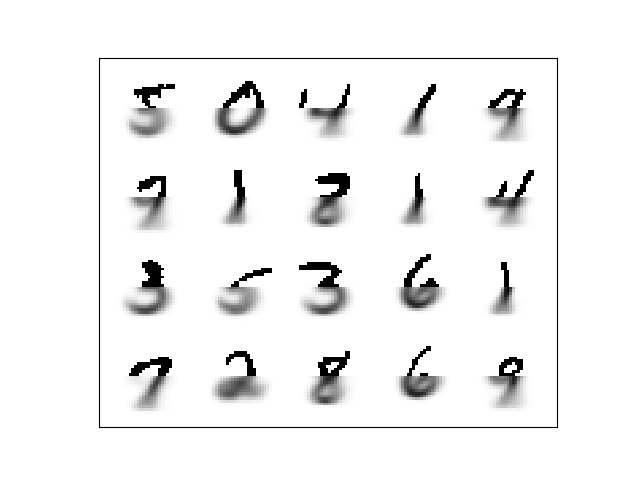
\includegraphics[width=0.75\linewidth]{q2f.jpg}
\label{fig:q2c}
\end{figure}
\end{homeworkProblem}
\clearpage
%----------------------------------------------------------------------------------------
%	PROBLEM 3
%----------------------------------------------------------------------------------------
\begin{homeworkProblem}

(a)\\
784 weights for each digit, 10 digit classes in total. 784 * 10 = 7840 parameters.\\

(b)\\
\begin{equation}
\begin{split}
\nabla_w log(p(c|\mathbf x, \mathbf w))
&= \nabla_w log(\frac{exp(\mathbf w^T_c \mathbf x)}{\sum_{c' = 0}^{9}exp(\mathbf w^T_{c'} \mathbf x)})\\
&= \nabla_w (log(exp(\mathbf w^T_c \mathbf x)) - log(\sum_{c' = 0}^{9}exp(\mathbf w^T_{c'} \mathbf x)))\\
&= \nabla_w (\mathbf w^T_c \mathbf x - log(\sum_{c' = 0}^{9}exp(\mathbf w^T_{c'} \mathbf x))) = F
\end{split}
\end{equation}
For c, 
\begin{equation}
\begin{split}
\frac{\partial F}{\partial w_{cd}} 
&= \frac{\partial}{\partial w_{cd}}  (\mathbf w^T_c \mathbf x - log(\sum_{c' = 0}^{9}exp(\mathbf w^T_{c'} \mathbf x))) \\
&= x_d - \frac{\partial}{\partial w_{cd}}(log(\sum_{c' = 0}^{9}exp(\mathbf w^T_{c'} \mathbf x)))\\
&= x_d - (\frac{exp(\mathbf w^T_{c} \mathbf x) x_d}{\sum_{c' = 0}^{9}exp(\mathbf w^T_{c'} \mathbf x)})\\
&= x_d - x_d \cdot p(c|\mathbf x, \mathbf w)
\end{split}
\end{equation}
For $\tilde c \neq c$,
\begin{equation}
\begin{split}
\frac{\partial F}{\partial w_{\tilde cd}} 
&= \frac{\partial}{\partial w_{\tilde cd}}  (\mathbf w^T_c \mathbf x - log(\sum_{c' = 0}^{9}exp(\mathbf w^T_{c'} \mathbf x))) \\
&= 0 - \frac{\partial}{\partial w_{\tilde cd}}(log(\sum_{c' = 0}^{9}exp(\mathbf w^T_{c'} \mathbf x)))\\
&= 0 - (\frac{exp(\mathbf w^T_{\tilde c} \mathbf x) x_d}{\sum_{c' = 0}^{9}exp(\mathbf w^T_{c'} \mathbf x)})\\
&= - x_d \cdot p(\tilde c|\mathbf x, \mathbf w)
\end{split}
\end{equation}
\clearpage
(c)\\
Code in q3.py. Notice that here, it is identical to using softmax with cross-entropy loss.
\begin{figure}[h!]
\centering
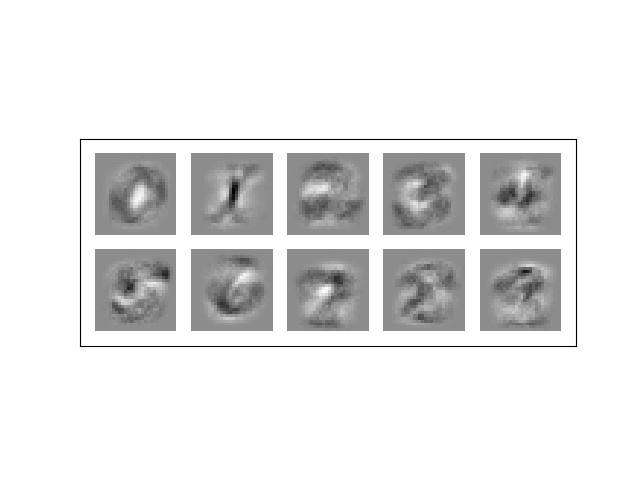
\includegraphics[width=0.75\linewidth]{q3c.jpg}
\label{fig:q2c}
\end{figure}

(d)\\
Training set accuracy: 0.9177\\
Training set average log prob: -0.312122612435\\
Test set accuracy: 0.8991\\
Test set average log prob: -0.359125675241\\
The accuracy and average log-likelihhood is better than the naive bayes's because using logistic regression, we drop the assumption that each pixel is independent.
\end{homeworkProblem}
\clearpage
%----------------------------------------------------------------------------------------
%	PROBLEM 4
%----------------------------------------------------------------------------------------

\begin{homeworkProblem}
(a)\\
$\theta$ : 784 * K params\\
$\pi$: K params (K-1 params strictly, since $\pi$ should sum to 1)\\
Total: 785K params (If we use K-1, the total would be 785K - 1)\\

(b)\\
$$
log(p(\mathbf x|\theta, \pi)) 
= log(\sum_{c=1}^{k} \pi_c \prod_{d=1}^{784}\theta_{cd}^{x_d}(1-\theta_{cd})^{(1-x_d)}) = F
$$

For an arbitray c', d':
\begin{equation}
\begin{split}
\frac{\partial F}{\partial \theta_{c'd'}} 
&= \frac{\partial}{\partial \theta_{c'd'}}  log(\sum_{c=1}^{k} \pi_c \prod_{d=1}^{784}\theta_{cd}^{x_d}(1-\theta_{cd})^{(1-x_d)}) \\
&= \frac{1}{\sum_{c=1}^{k} \pi_c \prod_{d=1}^{784}\theta_{cd}^{x_d}(1-\theta_{cd})^{(1-x_d)}} \frac{\partial}{\partial \theta_{c'd'}}(\sum_{c=1}^{k} \pi_c \prod_{d=1}^{784}\theta_{cd}^{x_d}(1-\theta_{cd})^{(1-x_d)})\\
&= \frac{1}{\sum_{c=1}^{k} \pi_c \prod_{d=1}^{784}\theta_{cd}^{x_d}(1-\theta_{cd})^{(1-x_d)}} \frac{\partial}{\partial \theta_{c'd'}}(\pi_{c'} \prod_{d=1}^{784}\theta_{c'd}^{x_d}(1-\theta_{c'd})^{(1-x_d)})\\
&= \frac{\pi_{c'} \prod_{d=1, d \neq d'}^{784}\theta_{c'd}^{x_d}(1-\theta_{c'd})^{(1-x_d)}}{\sum_{c=1}^{k} \pi_c \prod_{d=1}^{784}\theta_{cd}^{x_d}(1-\theta_{cd})^{(1-x_d)}} \frac{\partial}{\partial \theta_{c'd'}}(\theta_{c'd'}^{x_{d'}}(1-\theta_{c'd'})^{(1-x_{d'})})\\
&= \frac{\pi_{c'} \prod_{d=1, d \neq d'}^{784}\theta_{c'd}^{x_d}(1-\theta_{c'd})^{(1-x_d)}}{\sum_{c=1}^{k} \pi_c \prod_{d=1}^{784}\theta_{cd}^{x_d}(1-\theta_{cd})^{(1-x_d)}} (x_{d'}\theta_{c'd'}^{(x_{d'} - 1)}(1-\theta_{c'd'})^{(1-x_{d'})}-(1-x_{d'})(1-\theta_{c'd'})^{-x_{d'}}\theta_{c'd'}^{x_{d'}})\\
\end{split}
\end{equation}
\clearpage
(c)\\
Code in starter.py\\
Compare to the previous ones from the supervised model, the $\theta$s here are not as decisive and clear. The previous $\theta$s are clearly correspond to a specific digit, while in here, some of the $\theta$s seems to the a mix of different digits. Also, since K = 30 in our case, by dividing the training set into 30 clusters, different ways of writing a digit has its own $\theta$ map.
\begin{figure}[h!]
\centering
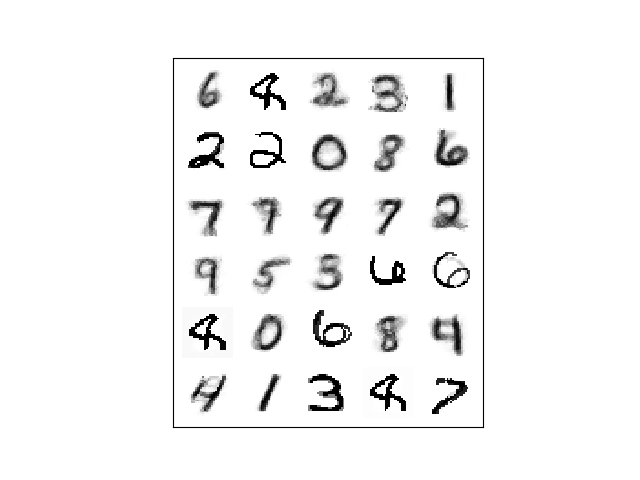
\includegraphics[width=0.6\linewidth]{q4plot.png}
\label{fig:q2c}
\end{figure}

(d)\\
Compare to the previous ones from the supervised model, the the generated bottom part here is actually not bad. Through more digits are paired with the bottom half from another digit, for the ones that are correct, the bottom half is more clear compare the the previous.
\begin{figure}[h!]
\centering
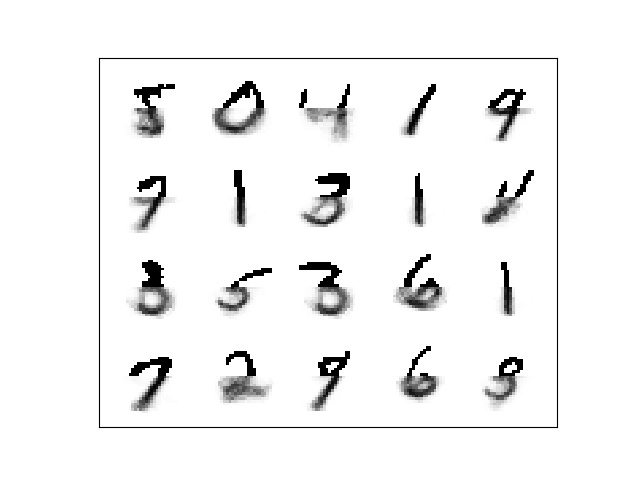
\includegraphics[width=0.6\linewidth]{q4d.jpg}
\label{fig:q2c}
\end{figure}
\end{homeworkProblem}
\clearpage
%----------------------------------------------------------------------------------------

\end{document}
